% !TEX root =  ../main_manuscript.tex 
\section{Introduction}
\label{c4:sec:introduction}
Chronic non-communicable diseases (e.g., cancer, lung, cardiovascular diseases) cause 60--70\% of human deaths worldwide~\citep{world2014global}. Often patients diagnosed with an early-stage disease undergo surveillance \emph{tests} to detect disease \emph{progression} timely. A progression is a non-terminal event, and usually a trigger for treatment and/or removal from surveillance. Benchmark tests used for confirming progression are usually \emph{invasive}, e.g., biopsies in prostate cancer surveillance~\citep{bokhorst2015compliance}, endoscopies in Barrett's esophagus~\citep{weusten2017endoscopic}, colonoscopies in colorectal cancer~\citep{krist2007timing}, and bronchoscopies in post lung transplant~\citep{mcwilliams2008surveillance} surveillance.

Invasive tests are repeated until progression is observed, typically as per a one-size-fits-all \emph{fixed schedule}, e.g., biannually,~\citep{krist2007timing,mcwilliams2008surveillance,bokhorst2015compliance}. A time gap between tests causes a time delay in detecting progression (Figure~\ref{c4:fig:1}). A shorter delay in detecting progression (\emph{benefit}) can provide a larger window of opportunity for curative treatment. However, with fixed schedules, this means conducting tests frequently. Frequent tests are \textit{burdensome} as they may cause pain and/or severe medical complications~\citep{krist2007timing,loeb2013systematic}. Consequently, patients may not always comply with frequent tests~\citep{bokhorst2015compliance, LeClercq2015325}. In general, because fixed schedules do not differentiate between fast and slow/non-progressing patients, they impose disproportionate burden/benefits across the patient population.

\begin{figure}
\centerline{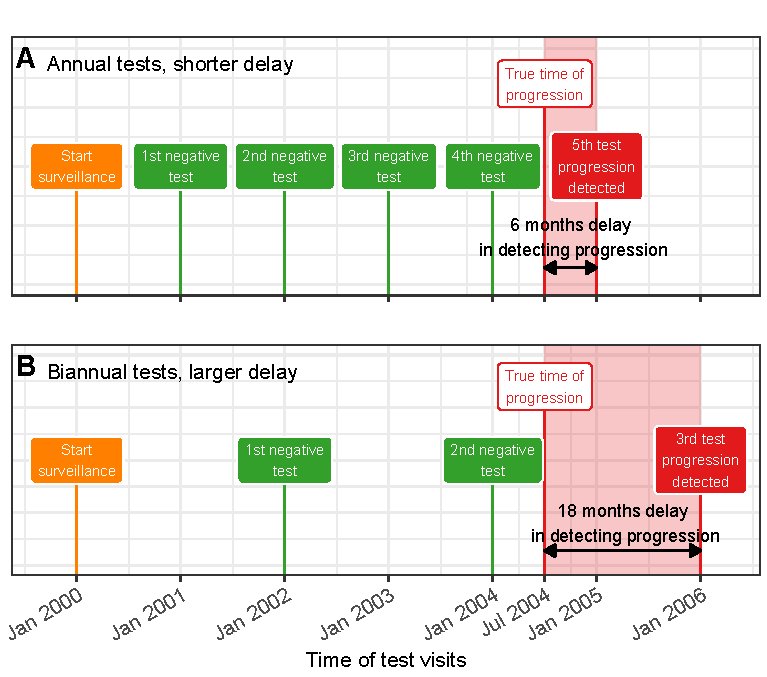
\includegraphics{contents/c4/images/c4_fig1.pdf}}
\caption{\textbf{Goal: Finding the optimal tradeoff between the number of invasive tests (burden) and time delay in detecting progression (shorter is beneficial)}. A progression is a non-terminal event in the surveillance of early-stage chronic non-communicable diseases. The true time of progression for the patient illustrated in this figure is July 2004. Since invasive tests are conducted repeatedly, progression is interval-censored and always observed with a delay. Frequent periodical invasive tests in \textbf{Panel~A} lead to a shorter time delay in detecting progression than infrequent periodical invasive tests in \textbf{Panel~B}. The interval-censored time of progression is Jan~2004--Jan~2005 in \textbf{Panel~A} and between Jan~2004--Jan~2006 in \textbf{Panel~B}.}
\label{c4:fig:1}
\end{figure}

The goal of this work (Figure~\ref{c4:fig:1}) is to optimize the number of invasive tests (burden) and the time delay in detecting progression (shorter is beneficial) better than fixed schedules. Specifically, we intend to \emph{personalize} test schedules using patients' clinical data accumulated over surveillance follow-up. This data includes baseline characteristics, previous test results, and longitudinal outcomes (e.g., biomarkers, medical imaging, physical examination). Many surveillance protocols currently personalize test schedules using heuristic methods such as decision flowcharts~\citep{bokhorst2015compliance,weusten2017endoscopic}. However, flowcharts discretize continuous outcomes, often exploit only the last measurement, ignore the measurement error in observed data, and plan only one test at a time. Alternatively, a complete personalized schedule of tests can be obtained using partially observable Markov decision processes or POMDPs~\citep{alagoz2010operations,steimle2017markov}. Although POMDPs typically discretize continuous longitudinal outcomes to avoid the curse of dimensionality. In scenarios such as ours, where decisions (test/no test) and disease state (low-grade disease/progressed) are both binary, POMDPs may not be necessary either. The reason is that such POMDPs give the same optimal schedule, which can be alternatively obtained by just planning a test when the probability of transition from non-progressed to progressed state is more than a certain threshold~\cite[see][Equation~1]{vickers2006decision}. 

Personalized schedules can also be obtained by optimizing an explicit utility function of the burden and/or benefit of a schedule. A challenge in this approach is quantifying burden and benefit. For a single test decision, \citet{tomer2019personalizedbiometrics} quantify the burden and benefit as the time difference by which the test undershoots (unnecessary test) or overshoots (delayed detection) the true progression time of a patient, respectively. Whereas, for a complete test schedule, \citet{bebu2017optimal} quantify burden as the number of tests planned (or their cost), and benefit as short time delay in detecting progression. Although, unlike the number of tests, the costs of time delay in detecting progression are not always quantifiable. For this issue, \citet{bebu2017optimal}, and \citet{vickers2006decision} have proposed scheduling tests when the risk of progression is above a threshold. Risk-based methodologies has also been explored by \citet{rizopoulos2015personalized}, and to evaluate the choice of risk thresholds \citet{wang2019learning} and \citet{tomer2019personalized} use measures of diagnostic accuracy (e.g., false-positive rate, true positive rate). However, a limitation of risk-based test decisions is that a single decision does not inform patients about the clinical consequences of continuing on surveillance. Also, measures of diagnostic accuracy are not personalized criteria for choosing risk thresholds.

We improve upon the works referenced above in many ways. Instead of a single risk-based test decision, we derive full risk-based test schedules that dynamically update with new clinical data over follow-up. Along with each schedule, we provide patients the clinical consequences of following it. Namely, the expected number of tests that will be required out of all planned tests to detect progression and the expected time delay in detecting progression. Unlike measures of diagnostic accuracy, we calculate these in a personalized manner. Also, these two are easily-quantifiable surrogates for important clinical aspects such as the window of opportunity for curative treatment, risk of adverse outcomes due to delayed detection of progression, financial costs of tests, risk of side-effects, and reduction in quality of life, etc. Our methodology is as follows. We first develop a full specification of the joint distribution of the patient-specific longitudinal outcomes and the time of progression. To this end, we utilize joint models for time-to-event and longitudinal data~\citep{tsiatis2004joint,rizopoulos2012joint} because they are inherently personalized. Specifically, joint models utilize patient-specific random effects~\citep{mcculloch2005generalized} to model longitudinal outcomes without discretizing them. Subsequently, we input clinical data of a new patient into the fitted model to obtain their predicted patient-specific cumulative-risk of progression at future visits. We then create personalized schedules by planning tests on future visits where this predicted cumulative-risk is above a particular \emph{threshold} (e.g., 5\% risk). We automate the choice of this threshold and the resulting schedule. In particular, we optimize a utility function of the expected number of tests (burden) and time delay in detecting progression (shorter is beneficial) for personalized schedules. We estimate these two quantities for any given schedule in a patient-specific manner using the patient's predicted risk profile. Hence, patients/doctors can compare the consequences of opting for personalized versus fixed schedules objectively.

Our motivation comes from the problem of scheduling biopsies in the world's largest prostate cancer surveillance study, called Prostate Cancer Research International Active Surveillance~\citep{bokhorst2015compliance}, or PRIAS. It has 7813 low/very-low grade cancer patients (1134 progressions, 104904 longitudinal measurements), many of whom are potentially over-diagnosed due to prostate-specific antigen (PSA) based screening~\citep{loeb2014overdiagnosis}. To reduce subsequent over-treatment, in surveillance, serious treatments (e.g., surgery, radiotherapy) are delayed until progression is observed. Surveillance involves regular monitoring of a patient's PSA (ng/mL), digital rectal examination or DRE (tumor shape/size), and biopsy Gleason grade group~\citep{epsteinGG2014}. Among these, a biopsy Gleason grade group~$\geq$ 2 is the reference test for confirming progression. Most often, biopsies are scheduled annually~\citep{loeb2014heterogeneity}. However, such a frequent schedule can put an unnecessary burden on patients with slow/non-progressing cancers and cause non-compliance~\citep{bokhorst2015compliance}. Since prostate cancer has the second-highest incidence among all cancers in males~\citep{GlobalCancerStats2012}, individualized biopsy schedules can reduce the burden of biopsies in numerous patients worldwide.

The remaining paper is as follows. Section~\ref{c4:sec:jointmodel} introduces the joint modeling framework. We describe the personalized scheduling methodology in Section~\ref{c4:sec:schedule}, and demonstrate them for prostate cancer surveillance patients in Section~\ref{c4:sec:results}. In Section~\ref{c4:sec:sim_study}, we compare personalized and fixed schedules via a simulation study based on a joint model fitted to the PRIAS dataset.